\section{A separate trained small-model posterior experiment}
\label{app:train04}
This experiment adapts a released 0.4B RWKV-7 initialization to an exactly specified binary conditional distribution. It is separate from the frozen F2 release, its checkpoints, and its long-context benchmark readings. The deployed tied bidirectional A1 model has 455,010,304 unique parameters. Each layer shares one recurrent mixer across the two scan directions; directional fusion and input-noise conditioning are included in the count. There are no hidden-depth loops or gate-modulation attachments in this arm. The output law is normalized over the two native bit-token rows (IDs 49 and 50), with a distinct mask ID 65535. Consequently these results concern a restricted binary generator, not free-text language-model quality.

\subsection{Known posterior, disjoint structures, and matched training}
Let $Y$ be uniform on $\mathbb F_2^8$ and condition on $(A,C)$, where $C=AY$ and $\operatorname{rank}(A)=4$. One family fixes four coordinates; the other imposes four disjoint pair-parity constraints. Both target posteriors are uniform on 16 vectors and have entropy four bits. Canonical labeled matrices are partitioned into train/development/test sets: 49/10/11 systematic structures and 73/16/16 pair-parity structures. The partitions are disjoint and exhaustive within their families. Targets, surface labels and equation order are randomized independently. Record identifiers are excluded from model inputs. This is held-out labeled-structure testing within two known families, not generalization to unseen algebraic topologies.

Three full-model runs use identical hashed initial weights and initialization seed zero, with separate data/corruption seeds 17, 29 and 43. Each uses 500 AdamW updates, global batch 32, learning rate $10^{-4}$, weight decay 0.01, gradient clipping at 1, FP32 master weights and optimizer states, and BF16 autocast. An eight-GPU, 20-update qualification checks execution, gradients and dtypes before the full runs; those updates are discarded. All fixed terminal checkpoints are retained. Each full run sees 16,000 examples.

The training law matches the absorbing objective: $t$ is uniform on $\{1,\ldots,8\}$; each target coordinate is independently masked with probability $t/8$; the prefix is clamped; and the estimator is
\begin{equation}
\widehat{\mathcal L}(\theta)=\frac{8}{tN}\sum_{i:X_t^i=\mask}-\log q_\theta^i(Y_i\mid X_t,t,A,C),\qquad N=8.
\end{equation}
Empty masks contribute differentiable zero and are not resampled. The exact-posterior expected objectives are $\tfrac12\log 2$ and $\tfrac9{16}\log 2$ for the two families, respectively; their equal mixture has optimum $\tfrac{17}{32}\log 2\approx0.368234$ nats per target token. An always-fair predictor instead has expected loss $\log 2$.

\subsection{Sampling and schedule-specific error accounting}
All policies use temperature one and the same terminal checkpoint within each seed. We compare one-round independent reveal; an oracle-matrix information-set two-round policy; a random-halves two-round policy; Bernoulli reveals at two, four and eight stages; and eight-round sequential sampling. Both two-round policies make exactly two neural calls and reveal four coordinates per call. The information-set policy uses $A$ to identify independent free coordinates, but never substitutes an algebraically solved output or accesses the sampled gold vector.

For a fixed ordered reveal partition $\pi=(J_1,\ldots,J_K)$, let $S_k=\bigcup_{j<k}J_j$. The KL chain rule yields
\begin{align}
\KL(P\Vert Q_{\theta,\pi})
&=D_\pi+E_{\theta,\pi},\\
D_\pi&=\sum_k\E_P\,\operatorname{TC}_P(Y_{J_k}\mid Y_{S_k},A,C),\\
E_{\theta,\pi}&=\sum_k\sum_{i\in J_k}\E_P\KL\!\left(P(Y_i\mid Y_{S_k},A,C)\Vert q_\theta^i(\cdot\mid Y_{S_k},A,C)\right).
\end{align}
This is a diagnostic application of the chain rule, not a new general cost identity; related conditional-total-correlation identities and dependence-adaptive schedules are studied by \citet{ctcdepth2026,intrinsicdependence2026}. The information-set policy has $D_\pi=0$. For pair parities, a pair contributes $\log2$ precisely when both coordinates are revealed in the same round; systematic posteriors incur no dependence cost. Lower dependence cost alone need not imply a better learned sampler: information-set sampling improves forward KL over random halves exactly when $E_{\theta,\mathrm{info}}-E_{\theta,\mathrm{random}}<D_{\mathrm{random}}$.

Each family has 16 locked test conditions with 32 draws per policy. A separate 64-condition calibration panel per family covers all eight corruption stages and measures exact oracle marginal KL, deterministic-bit accuracy, and fair-bit calibration. Fixed-policy endpoint KL is computed directly using stable log probabilities and all 16 valid outputs on a small audit of two conditions per family. Marginal calibration under the training corruption law is not identified with schedule-specific $E_{\theta,\pi}$. For Bernoulli policies, a sampled path probability is not an endpoint probability; endpoint joint KL is not reported for the trained model.

The mean losses over the final 100 updates are 0.6965, 0.7018 and 0.7008 for seeds 17, 29 and 43, respectively, close to the always-fair baseline rather than the oracle optimum. Held-out deterministic-bit accuracy ranges from 47.62--52.38\% for systematic constraints and 49.68--50.32\% for pair parities. The copied mixer matches the installed FLA 0.5.0 attention implementation bit-for-bit in first- and last-layer preflights on all evaluation ranks; this does not establish official-kernel parity. Execution qualification therefore passed while conditional task competence did not emerge under this recipe.

\subsection{Measured outcomes}
All three terminal checkpoints are included. Table~\ref{tab:train04competence} separates denoiser competence from the two-call policy comparison. Table~\ref{tab:train04samplers} reports equal-seed descriptive means; full seed-specific results and source hashes are retained in the accompanying receipts.
\begin{table}[htbp]
\centering\small
\setlength{\tabcolsep}{4pt}
\caption{Held-out competence and sampling, by training seed. Accuracy and validity are percentages; marginal KL is in nats per masked bit. The denoiser calibration panel is separate from the sampling conditions.}
\label{tab:train04competence}
\begin{tabular}{@{}rlrrrrr@{}}
\toprule
Seed & Family & Det. acc. & Marg. KL & Info valid & Random valid & One valid\\
\midrule
17 & Systematic & 47.62 & 0.360 & 6.45 & 7.42 & 5.47\\
17 & Pair parity & 50.32 & 0.201 & 6.45 & 3.52 & 5.66\\
29 & Systematic & 52.38 & 0.350 & 7.62 & 9.18 & 6.45\\
29 & Pair parity & 49.68 & 0.197 & 7.62 & 5.08 & 6.25\\
43 & Systematic & 47.62 & 0.358 & 6.25 & 7.62 & 5.66\\
43 & Pair parity & 50.32 & 0.200 & 6.45 & 3.91 & 6.05\\
\bottomrule
\end{tabular}
\end{table}
For systematic, the equal-seed information-set minus random-halves validity difference is -1.30 percentage points, with paired condition-bootstrap95\% interval $[-3.91,1.24]$. The interval conditions on the three fitted checkpoints.
For paired parity, the equal-seed information-set minus random-halves validity difference is 2.67 percentage points, with paired condition-bootstrap95\% interval $[0.39,5.01]$. The interval conditions on the three fitted checkpoints.
\begin{table}[htbp]
\centering\small
\caption{Equal-seed decoder means. Coverage is the fraction of the 16 valid vectors observed among 32 draws per condition. Collision is the fraction of distinct draw pairs with identical outputs. Joint KL uses only two audit conditions per family and is not estimated for Bernoulli policies.}
\label{tab:train04samplers}
\begin{tabular}{@{}llrrrrr@{}}
\toprule
Family & Policy & Valid (\%) & Coverage (\%) & Collision (\%) & NFE & Joint KL\\
\midrule
Systematic & One round & 5.86 & 10.94 & 0.48 & 1.00 & 2.823\\
Systematic & Info set (2) & 6.77 & 12.76 & 0.35 & 2.00 & 2.825\\
Systematic & Random halves (2) & 8.07 & 16.15 & 0.37 & 2.00 & 2.828\\
Systematic & Bernoulli (2) & 6.71 & 12.76 & 0.43 & 2.00 & ---\\
Systematic & Bernoulli (4) & 5.92 & 11.33 & 0.43 & 3.92 & ---\\
Systematic & Bernoulli (8) & 5.86 & 10.16 & 0.50 & 7.48 & ---\\
Systematic & Sequential (8) & 5.79 & 10.55 & 0.41 & 8.00 & 2.826\\
Pair parity & One round & 5.99 & 11.33 & 0.39 & 1.00 & 2.823\\
Pair parity & Info set (2) & 6.84 & 13.15 & 0.42 & 2.00 & 2.825\\
Pair parity & Random halves (2) & 4.17 & 8.20 & 0.48 & 2.00 & 2.825\\
Pair parity & Bernoulli (2) & 6.38 & 11.85 & 0.40 & 2.00 & ---\\
Pair parity & Bernoulli (4) & 5.92 & 11.20 & 0.50 & 3.90 & ---\\
Pair parity & Bernoulli (8) & 4.82 & 8.98 & 0.47 & 7.53 & ---\\
Pair parity & Sequential (8) & 5.47 & 9.51 & 0.50 & 8.00 & 2.826\\
\bottomrule
\end{tabular}
\end{table}
\begin{figure}[htbp]
\centering
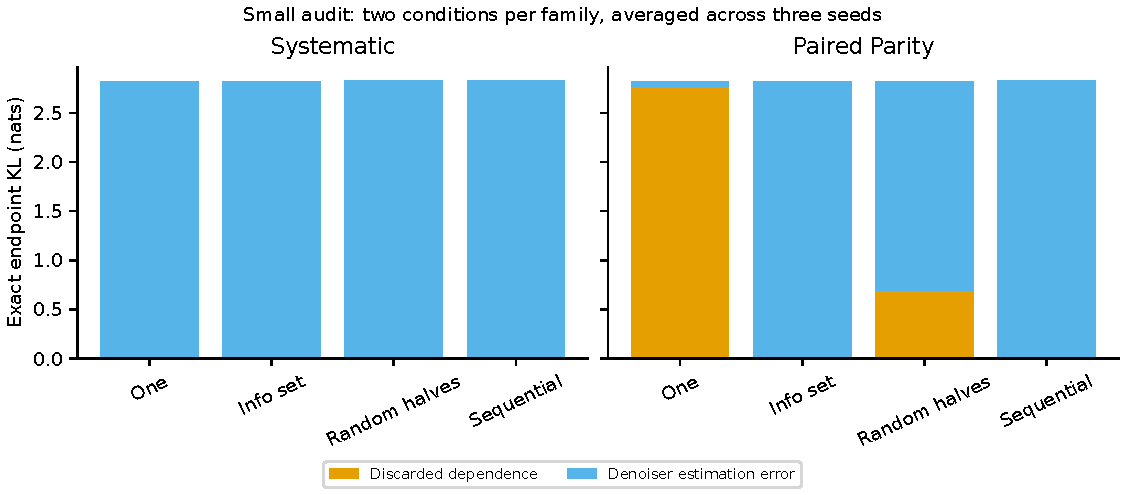
\includegraphics[width=\linewidth]{results/train04/final/figures/kl_decomposition.pdf}
\caption{Exact fixed-policy endpoint KL split into discarded dependence and denoiser estimation error on the small audit panel. The bars average the same two conditions per family across all three training seeds.}
\label{fig:train04decomposition}
\end{figure}

\paragraph{Post-primary exact-probability diagnostic.}
The sampled parity contrast motivated an additional diagnostic, without changing any checkpoint, hyperparameter or sampler. We enumerated all 16 valid endpoint probabilities for both two-round policies on all 32 existing test conditions per checkpoint. This removes Monte Carlo error in finite-panel validity, but does not remove uncertainty about unseen conditions. Audit memoization is not a decoding-speed measurement.
\begin{table}[htbp]
\centering\small
\caption{Post-primary exact model expectations, equal-seed means on the existing conditions. The sampled tables above are retained unchanged.}
\label{tab:train04exact}
\begin{tabular}{@{}lrrrrr@{}}
\toprule
Family & Info valid (\%) & Random valid (\%) & Difference (pp) & Info KL & Random KL\\
\midrule
Systematic & 6.0300 & 6.0288 & 0.0012 & 2.8537 & 2.8540\\
Pair parity & 6.3004 & 6.3000 & 0.0004 & 2.8243 & 2.8243\\
\bottomrule
\end{tabular}
\end{table}

Cross-execution checking found joint-KL differences up to 0.00970 nats on overlapping audit conditions. The enumerated values therefore remove endpoint Monte Carlo error but do not establish reproducibility at the precision of the tiny reported policy differences; numerical qualification remains pending.


The low validity and near-chance calibration do not demonstrate the proposed useful learned sampling advantage. In the primary small KL audit, the information-set policy eliminates oracle dependence cost but incurs about 2.82 nats of denoiser estimation error. This is a negative training pilot, not a refutation of the exact-posterior construction or evidence that the architecture cannot learn the task under another recipe.

\subsection{A policy-specific training objective}
For a fixed reveal policy, the error decomposition suggests a direct population objective. Draw a target history from $P$ and a round $k$ with probability $\rho_k>0$, construct the exact decoder canvas (including its time code), and use true marginal soft targets $p_i=P(Y_i\mid Y_{S_k},A,C)$. Define
\begin{equation}
\mathcal L_\pi(\theta)=\E_{Y,k}\left[\frac{1}{N\rho_k}\sum_{i\in J_k}\operatorname{CE}(p_i,q_\theta^i)\right].
\end{equation}
Writing $\mathcal H_\pi$ for the same expression with conditional entropy in place of cross-entropy gives
$N(\mathcal L_\pi-\mathcal H_\pi)=E_{\theta,\pi}$: expand cross-entropy as entropy plus marginal KL and cancel $\rho_k$ in the round expectation. For the information-set policy, this is the endpoint forward KL itself. If $v$ is the model probability of the valid coset, then
$\KL(P\Vert Q)=-\log v+\KL(P\Vert Q(\cdot\mid\mathrm{valid}))$,
so $v\geq\exp[-N(\mathcal L_\pi-\mathcal H_\pi)]$. These are population statements for the same condition distribution, not finite-sample guarantees or newly claimed general identities. High validity alone leaves the second, within-support diversity term unconstrained.

The ordinary corruption objective need not tightly control this quantity. At $N=8$, the specified four-coordinate mask in the second information-set round at stage 4 receives probability $(1/8)2^{-8}$ and loss weight $8/(4N)=1/4$. Its error sum therefore enters corruption excess with coefficient $1/8192$; the first-round error enters with coefficient at least $1/64$. Nonnegativity yields only the conservative bound $E_{\theta,\mathrm{info}}\leq8192\,\mathcal L_{\mathrm{corruption,excess}}$. This motivates testing policy-history supervision, without attributing the negative pilot to mask coverage. Exact marginal soft labels are privileged synthetic supervision. This objective has not yet been evaluated in a trained confirmatory experiment.

A mixture can improve objective coverage explicitly. Let $\mathcal L_{\mathrm{mix}}=(1-\alpha)\mathcal L_{\mathrm{corruption}}+\alpha\mathcal L_\pi$, with $\alpha>0$, and let $\mathcal H_{\mathrm{mix}}$ be its corresponding oracle entropy baseline. Nonnegative marginal KL gives $E_{\theta,\pi}\leq (N/\alpha)(\mathcal L_{\mathrm{mix}}-\mathcal H_{\mathrm{mix}})$. For information-set sampling this also bounds endpoint KL. At $N=8$ and $\alpha=1/2$, the coefficient is 16. This is an objective-coverage guarantee, not an optimization or finite-sample guarantee; the matched four-bit and terminal eight-bit mixture ablations below have completed. In its policy branch, the canvas masks all unrevealed coordinates while the loss scores only the coordinates revealed in the sampled round.

\paragraph{A sufficient optimization target.}
For $N=2m$ disjoint parity pairs, a uniformly random balanced two-round partition puts the two coordinates of each pair in the same round with probability $(m-1)/(2m-1)$. Its expected dependence cost is therefore $\overline D_{\mathrm{random}}=m(m-1)\log2/(2m-1)$. Write $\delta_{\mathrm{par}}$ for population mixture excess conditioned on the parity family, with $\alpha=1/2$. Since information-set endpoint KL is at most $2N\delta_{\mathrm{par}}$ and random-policy estimation error is nonnegative, $2N\delta_{\mathrm{par}}<\overline D_{\mathrm{random}}$ suffices for an advantage in expected endpoint KL over a uniform random balanced partition. At $N=8$, the threshold is $\delta_{\mathrm{par}}<(3/28)\log2\approx0.07427$. If only equal-family mixture excess $\delta$ is available, nonnegativity gives $\delta_{\mathrm{par}}\leq2\delta$, and the sufficient threshold becomes $\delta<(3/56)\log2\approx0.03713$. These conservative population targets are not achieved results, necessary conditions, guarantees from observed minibatch losses, or claims about every fixed random partition. In particular the comparison is uninformative at $N=2$, where every balanced split separates the sole pair and both policies have zero dependence cost. Enumeration of all balanced partitions for $N\in\{2,4,6,8,10,12\}$ verifies the combinatorial expectation.

\paragraph{Numerical follow-up.}
A separate probe repeats eight canvases six times in alternating order, with two processes for each of four precision configurations, on the seed-43 checkpoint. All repeated within-process logits agree exactly and parameter hashes remain unchanged. The largest paired cross-process logit difference is $0.046875$ in the BF16 configuration with PyTorch TF32 disabled, versus $7.15\times10^{-6}$ in FP32; the other two paired configurations agree on these inputs. This limited probe does not establish a kernel-level cause or general reproducibility. It supports retaining numerical qualification on the tiny endpoint contrasts and using FP32 in subsequent development.

A subsequent recurrence-only diagnostic compares FP32-input chunk outputs and all six input gradients against an explicit double-precision scan on three bounded synthetic inputs (lengths 65, 117 and 128, head dimension 64). Maximum relative $\ell_2$ discrepancies are 0.001385 for outputs and 0.003153 for gradients, with all tested values finite. Disabling PyTorch TF32 does not set Triton's dot-product precision: the inspected local Triton backend defaults unqualified dot products to TF32. Thus FP32 parameter and activation dtypes alone should not be described as an IEEE-precision arithmetic guarantee. On the same probe inputs, setting \texttt{TRITON\_F32\_DEFAULT=ieee} with a fresh kernel cache reduces maximum output and gradient relative errors to $2.26\times10^{-7}$ and $4.84\times10^{-7}$, respectively. This supports a precision explanation for these probe discrepancies; it does not establish equivalence of the complete model to official RWKV kernels. The matched curriculum runs retain their original common numerical configuration.

\subsection{First curriculum development phase}
After the negative pilot, a matched development comparison changes both arms to FP32 tensors, a binary log-odds head, learning rate $3\times10^{-5}$ with 50-update warmup, and a fixed 2--4--8-bit curriculum. One arm uses sampled hard labels; the other uses exact conditional marginal soft labels with the same corruption weighting. The first phase is now complete: 300 updates on two-bit tasks, one initialization and data seed, with optimizer state retained. The original eight-bit task is unchanged and has not yet received curriculum training. These development results are not a confirmatory test or an isolated ablation of every change from the primary pilot.
\begin{table}[htbp]\centering\small
\caption{Completed two-bit curriculum phase. Marginal KL is per masked bit on the common development panel, not schedule-specific endpoint KL.}
\begin{tabular}{@{}llrr@{}}\toprule
Objective & Dimension & Deterministic accuracy (\%) & Marginal KL\\\midrule
Hard labels & 2 & 100.00 & 0.047179\\
Hard labels & 8 & 58.67 & 1.373374\\
Conditional soft labels & 2 & 100.00 & 0.000733\\
Conditional soft labels & 8 & 58.23 & 3.412035\\
\bottomrule\end{tabular}\end{table}
Both arms attain perfect thresholded accuracy on this two-bit panel, while soft targets have lower proper loss. Eight-bit calibration deteriorates during this first phase; the result therefore demonstrates learning of the small curriculum task, not the terminal sampling mechanism or cross-size generalization. Later curriculum phases remain pending.

\paragraph{Endpoint audit of the first curriculum phase.}
On eight two-bit parity development conditions, hard-label information-set sampling has mean valid mass 58.438\% and endpoint KL 0.537734 nats; conditional-soft-label sampling has 99.914\% valid mass and KL 0.002346 nats. One-round soft-label sampling instead has 50.017\% valid mass and KL 0.695689 nats, including the unavoidable $\log2$ dependence cost. The independent marginal-error sums agree with the endpoint decomposition. The eight two-bit parity condition draws cover four unique prompts and one pair structure; this is a competence diagnostic, not held-out-structure generalization. This small-task result distinguishes thresholded accuracy from sampling fidelity. It does not demonstrate an information-set advantage over random halves: with only one parity pair, either one-coordinate-per-round ordering has zero dependence cost. Soft-label random halves likewise has 99.957\% valid mass on this panel.

On the original eight-bit parity development panel before eight-bit curriculum training, information-set valid mass remains 6.193\% for hard labels and 6.733\% for soft labels, with endpoint KL 7.2954 and 18.8652 nats, respectively. The large conditional-within-valid-support errors show that similar validity can conceal very different posterior mismatch. The full development audit retains both families, all three dimensions, and all three fixed policies, rather than selecting only the successful two-bit slice.

\subsection{Four-bit curriculum audit: competence and forgetting}
At the fixed 700-update curriculum boundary, both ordinary-corruption objectives achieve approximately 83\% deterministic-bit accuracy when the two families are pooled. Exact information-set sampling reveals a different family-level result (Table~\ref{tab:dev700exact}): systematic constraints are almost always satisfied at $N=4$, whereas paired-parity validity remains near its $2^{-N/2}$ chance baseline. At $N=2$, parity validity has returned to approximately 50\%, including for the soft-target model whose 300-update checkpoint attained 99.91\%. Thus the earlier small-task success was not retained during the four-bit curriculum. These are fixed development checkpoints from one data seed, not confirmatory replications. The $N=8$ rows are transfer diagnostics before the terminal eight-bit training phase; they do not replace that phase.

\begin{table}[ht]
\centering\small
\begin{tabular}{llrrr}
\toprule
Objective & Family & $N$ & Endpoint KL & Valid mass (\%) \\
\midrule
Hard & Parity & 2 & 0.6971 & 50.002 \\
Hard & Systematic & 2 & 0.0042 & 99.952 \\
Hard & Parity & 4 & 1.3961 & 24.965 \\
Hard & Systematic & 4 & 0.0120 & 99.862 \\
Hard & Parity & 8 & 2.7937 & 6.229 \\
Hard & Systematic & 8 & 2.7207 & 48.931 \\
Soft & Parity & 2 & 0.6956 & 50.002 \\
Soft & Systematic & 2 & 0.0012 & 100.000 \\
Soft & Parity & 4 & 1.3931 & 24.979 \\
Soft & Systematic & 4 & 0.0048 & 100.000 \\
Soft & Parity & 8 & 2.7874 & 6.235 \\
Soft & Systematic & 8 & 15.2007 & 22.338 \\
\bottomrule
\end{tabular}
\caption{Exact development information-set sampling at update 700. Each row averages eight condition draws; valid outputs are enumerated exactly. Dependence cost is zero, so all reported endpoint KL is denoiser estimation error. Small-dimension condition draws can repeat prompts and structures, as in the preceding curriculum audit.}
\label{tab:dev700exact}
\end{table}


The matched 50/50 policy-history mixture also fails to recover four-bit parity competence at update 700. Information-set validity is 24.878\% with hard targets and 24.999\% with soft targets, with endpoint KL of 1.4197 and 1.3873 nats respectively (the always-fair baseline is $\log4\approx1.3863$). Systematic validity is 99.990\% and 99.999\%. Both models also return to approximately 50\% two-bit parity validity. These exact audits use the same development conditions as the ordinary-corruption arms and preserve the paired 300-update parent checkpoints. Thus policy coverage and privileged soft labels are not sufficient to produce the intended neural computation under this four-bit training budget. The bound on the population objective remains valid, but these outcomes do not establish useful posterior learning. The soft-target mixture does have a descriptive 0.03557-nat KL advantage over the fixed random-halves panel (validity 24.999\% versus 24.311\%); this contrast is reported rather than treated as zero, but information-set performance remains near the 25\% always-fair baseline. All four declared arms subsequently complete the original eight-bit terminal phase reported below; no confirmation panel is used for this decision.


\paragraph{Why oracle dependence reduction can cancel.}
If each prediction is history- and round-independent, $q_\theta^i(y_i\mid Y_{S_k},k,c)=q_\theta^i(y_i\mid c)$, every ordered reveal partition has the same endpoint law $Q_\pi(y\mid c)=\prod_iq_\theta^i(y_i\mid c)$: multiply the per-round factors and note that each coordinate occurs once. Thus endpoint KL is invariant even when $D_\pi$ changes, because $E_\pi=\KL(P\Vert Q)-D_\pi$. For an always-fair predictor on $m$ disjoint parity pairs, this gives $\KL(P\Vert Q)=m\log2$, valid mass $2^{-m}$, and $E_\pi=m\log2-D_\pi$. This elementary consequence of the product law is a diagnostic, not a new general theorem or proof that the learned predictors are exactly history-independent.

On the four-bit audit's fixed random partitions, mean $D_{\mathrm{random}}=0.173287$ nats. The corresponding $E_{\mathrm{info}}-E_{\mathrm{random}}$ values are 0.173197 and 0.173326 for ordinary hard and soft training, and 0.173258 and 0.137713 for mixture hard and soft training. Therefore the first three arms almost exactly cancel the oracle dependence reduction, while the fourth retains the modest descriptive contrast reported above. This panel's mean dependence cost is not the uniform-partition population expectation used in the sufficient optimization target. Finite checks at $N=2,4,8$ verify schedule invariance for both fair and biased history-independent predictors.

\subsection{Completed eight-bit development endpoints}
All four declared development arms complete 1500 updates, including 800 updates on the original eight-bit task, and retain their fixed terminal checkpoints. Each exact audit contains 144 condition-policy records across three dimensions, plus 48 history-response records. Table~\ref{tab:terminaln8} reports the terminal $N=8$ information-set results. None learns the paired-parity posterior: validity is near its 6.25\% always-fair baseline, while endpoint KL remains near or above $4\log2\approx2.7726$. The ordinary arms and soft-target mixture nearly solve direct systematic constraints, but their positive within-valid KL shows that high validity is not posterior fidelity. The hard-label mixture also loses much of that direct-constraint competence.

\begin{table}[ht]
\centering\small
\begin{tabular}{lllrrr}
\toprule
Training & Labels & Family & Endpoint KL & Valid (\%) & Within-valid KL \\
\midrule
Ordinary & Hard & Parity & 2.8007 & 6.219 & 0.0230 \\
Ordinary & Hard & Systematic & 0.3022 & 99.932 & 0.3016 \\
Ordinary & Soft & Parity & 2.7897 & 6.226 & 0.0132 \\
Ordinary & Soft & Systematic & 0.2726 & 100.000 & 0.2726 \\
Mixture & Hard & Parity & 2.9057 & 6.103 & 0.1067 \\
Mixture & Hard & Systematic & 2.4272 & 13.350 & 0.0318 \\
Mixture & Soft & Parity & 2.9506 & 6.059 & 0.1425 \\
Mixture & Soft & Systematic & 0.0802 & 99.997 & 0.0802 \\
\bottomrule
\end{tabular}
\caption{Fixed 1500-update development endpoints, one data seed and eight condition draws per family. All rows use the same information-set policy with zero dependence cost. These are controlled development comparisons from paired 300-update parents, not four independent pretrained initializations or confirmatory replications.}
\label{tab:terminaln8}
\end{table}

To measure use of revealed history, hold the public condition and all other free bits fixed, flip one revealed free bit, and measure the signed change in the predicted probability of its parity partner's newly correct value. Averaging over all such feasible information-set histories gives response 1 for the oracle and 0 for any history-independent predictor. This is twice the mean correct-class probability on these dependent coordinates minus one, not an independent error certificate. Predictions are reused from the exact audit cache, adding no model calls. All four terminal paired responses have absolute value below $1.4\times10^{-5}$; the ordinary hard/soft and mixture-soft values have magnitude below $4\times10^{-7}$. Such tiny values do not establish a reversed rule or a reproducible sign. The models are effectively unresponsive on this diagnostic despite substantially higher aggregate deterministic accuracy in three arms.

A separate full-model audit of the ordinary hard checkpoint with explicit Triton IEEE arithmetic preserves the parity failure (6.219\% information-set validity and approximately 2.80068 nats endpoint KL). The trained input embeddings of tokens 0 and 1 remain distinct. These checks do not support simple embedding collapse or the tested arithmetic precision as explanations for the qualitative failure; they do not exclude other implementation defects, certify official-kernel parity, or establish repeated-process reproducibility. The results motivate a separate public-label serialization diagnostic, not a positive claim for the present training recipe. Fresh-seed confirmation remains unexecuted.


\subsection{Scope of the evidence}
Constraint validity does not certify posterior fidelity: a collapsed generator can return one valid vector indefinitely. We therefore also report valid support coverage and collision concentration. With 32 independent draws, the perfect uniform posterior has expected coverage $1-(15/16)^{32}\approx87.32\%$ and collision probability $1/16$. The initial pilot's three fitted models provide three training replicates; condition-bootstrap intervals remain conditional on these checkpoints and do not estimate population-level training uncertainty precisely. The small exact-KL panel is diagnostic. The public $(A,C)$ prompt remains on the full input canvas; this is not a measurement of information stored in a learned compressed recurrent state. These results do not establish long-context retention, a learned dependency selector, official-RWKV kernel parity, free-language quality, or a new neural-architecture advantage.

\paragraph{Public-label serialization diagnostic.}
A separate soft-target comparison retains the original equations and output order, but places the public variable name beside each answer slot. Both ordinary and mixture arms restart from their matched 300-update model and optimizer; labels introduce no additional answer information but add four native tokens per target. Over updates 301--700, each label-format arm processes 1,177,600 training input tokens versus 972,800 for the reconstructed original format (21.1\% more); these comparisons match examples and updates, not input-token compute. At update 700, exact four-bit information-set validity remains 24.970\% and 24.956\%, with KL 1.39469 and 1.40815 nats, respectively. Signed parity-partner responses have magnitude below $1.3\times10^{-5}$ in both arms. Four-bit systematic KL is 0.00523 and 0.00017 nats. Thus explicit slot labels do not recover the required parity conditional at this checkpoint. Before eight-bit training, the label format improves systematic-task transfer KL from 15.2007 to 0.01019 nats under ordinary masking and from 14.9818 to 2.32040 nats under mixture masking, while parity transfer remains poor. This is evidence of a task-specific representation benefit, not the intended parity computation. At update 1500, both exact eight-bit audits remain negative for parity: ordinary/mixture information-set validity is 6.061\%/6.069\%, with endpoint KL 2.94585/2.93842 nats. Signed partner responses are approximately $-5.6\times10^{-8}$/$-1.2\times10^{-6}$, which do not establish useful history use or a meaningful negative sign. Systematic-task KL is 0.08549/0.07265 nats with validity above 99.9999\%. Thus the representation change improves some copying-task outcomes but does not recover the required parity computation. These are single-seed development results; fresh-seed confirmation remains unexecuted.

\paragraph{Completed paired-history development comparison.}
To test whether training-history coupling helps recover the missing dependence on revealed values, two further arms share the label-mixture terminal checkpoint and optimizer. Both use only information-set policy histories, a uniform choice of its two rounds, and exact marginal soft targets; their population excess objective is $E_{\theta,\mathrm{info}}/N$. Each update uses 16 public conditions, balanced across families, and two histories per condition (32 document forwards). The control draws both free-bit assignments independently. The complementary arm draws one uniformly and complements all free bits for the second, completing the dependent coordinates within the same public affine constraint. Both members remain uniform under the same conditional law. Public conditions, reveal rounds, first histories, input-token counts, model, optimizer, and learning rate match between arms; only the second-history coupling changes. Two 20-update GPU qualification runs passed and are discarded. Research restarts from the common pre-probe checkpoint, with fixed audits after 400 and 1000 additional updates on the original eight-bit task. Both prespecified 1000-update continuations have completed, each processing 4,768,000 input tokens over the additional training phase. Terminal checkpoint hashes and all 1000 finite update records were verified. Table~\ref{tab:pairedhistory} reports both fixed checkpoints.

\begin{table}[ht]
\centering\small
\caption{Exact eight-bit development endpoints for paired-history continuations (seed 17). KL is in nats. All columns use the information-set two-call policy; parity validity is a percentage. Each family has eight fixed development conditions. These use the common default Triton arithmetic, not the separate IEEE qualification.}
\label{tab:pairedhistory}
\begin{tabular}{rlrrr}
\toprule
Updates & Histories & Parity KL & Parity valid (\%) & Systematic KL \\
\midrule
400 & Independent & 2.78353 & 6.2366 & 0.005201 \\
400 & Complementary & 2.77272 & 6.2498 & 0.000078 \\
1000 & Independent & 2.80065 & 6.2189 & 0.013337 \\
1000 & Complementary & 2.77262 & 6.2500 & 0.000016 \\
\bottomrule
\end{tabular}
\end{table}


Complementary training approaches the fair-independent parity law ($\KL=\log16$, validity $1/16$). Its terminal signed partner response is $5.60\times10^{-9}$, versus $-6.42\times10^{-7}$ for independent histories; these do not establish useful partner dependence. The random-minus-information-set parity KL differences are $-2.38\times10^{-4}$ and $1.21\times10^{-6}$ nats, respectively. The latter tiny positive sign is not evidence of a useful scheduling advantage. The independent arm's systematic one-round and random-halves KLs are 2.83267 and 2.77467 nats, whereas the complementary arm remains below $1.58\times10^{-5}$ for these policies. The calibration difference therefore includes sensitivity to policies outside the supervised information-set objective. It does not establish accurate parity sampling.

The complementary-versus-independent comparison is now frozen for data/corruption seeds 53, 71, and 89. Each seed reconstructs the complete shared 1500-update curriculum from the released checkpoint with initialization seed zero, then forks model and optimizer into two fixed 1000-update branches. The questions are whether the calibration difference and parity failure persist, not whether a selected interim checkpoint can yield a positive result. All four sampling policies will be evaluated on the previously fixed 54-condition panel with explicit IEEE inference. All three parents have completed 1500 updates, each processing 5,524,800 training input tokens; their contiguous finite update records and terminal checkpoint hashes were verified. The six fixed-terminal branches are submitted, but no confirmation model has yet evaluated this panel. These pending replications are not endpoint results.

A subsequent full-model numerical qualification uses the complementary 400-update checkpoint with explicit \texttt{TRITON\_F32\_DEFAULT=ieee}, FP32 tensors, and PyTorch TF32 disabled. Eight GPU worker processes evaluate the same 12 development canvases (two conditions at each of $N=2,4,8$, in fully masked and information-set-visible rounds), repeating each production call three times. Within-process repeated log probabilities and direct-backbone versus serial-wrapper log probabilities agree exactly; the maximum cross-process absolute log-probability difference is $5.73\times10^{-6}$. These satisfy the predeclared $10^{-5}$ within-process/wrapper and $10^{-4}$ cross-process tolerances. The check concerns one checkpoint and a fixed canvas panel within one scheduler launch; it neither verifies training gradients nor establishes official-RWKV equivalence or stability on all inputs. No confirmation conditions are used.


The elementary antithetic calculation explains both the motivation and its limit. At fixed public condition and round, let $g(U)$ be a raw per-history gradient and $J$ complement the uniformly distributed free bits. Define $g_+=(g+g\circ J)/2$ and $g_-=(g-g\circ J)/2$. The involution preserves measure, so $\E g_-=0$ and the centered even and odd components have zero cross-covariance. Hence
\[
\operatorname{Cov}(g)=\operatorname{Cov}(g_+)+\operatorname{Cov}(g_-),\qquad
\operatorname{Cov}(\bar g_{\mathrm{comp}})-\operatorname{Cov}(\bar g_{\mathrm{iid}})
=\tfrac12\bigl[\operatorname{Cov}(g_+)-\operatorname{Cov}(g_-)\bigr].
\]
There is no universal variance ordering: for uniform sign bits $(s_1,s_2)$ and $g=(s_1s_2,s_1)$, this covariance difference is $\operatorname{diag}(1/2,-1/2)$. In the parity-dependent round, complementary histories have complementary target labels. For a history-independent binary logit $z$, their mean cross-entropy derivative is $\sigma(z)-1/2$, eliminating sampled-label imbalance in that shared-logit direction. This does not guarantee that a recurrent representation learns the necessary interaction. Equal mean raw gradients also do not imply equal mean updates after nonlinear gradient clipping or AdamW. These statements justify a controlled experiment, not a claimed general optimization improvement.


\paragraph{Analytical references for the frozen confirmation panel.}
After recipe selection was frozen, exact finite-posterior calculations verified the four reveal policies on the fixed panel without loading a neural model. Table~\ref{tab:confirmationoracle} gives the parity references. Both the oracle and initial-marginal product references are exact on the separate systematic family under every policy. The always-fair predictor instead has KL $\log16$ and validity $1/16$ on both families. The panel's mean random-halves dependence cost is 1.299651 nats, distinct from the uniform-partition population expectation and from the earlier development panel. Mean validity averages the condition-specific values $e^{-D_\pi(c)}$; it is not $e^{-\E D_\pi(c)}$. These controls check interpretation and endpoint accounting, not neural learning. No trained confirmation checkpoint has yet been evaluated.
\begin{table}[ht]
\centering\small
\caption{Analytical reference laws on the frozen confirmation parity panel (32 conditions over 16 structures). These are not trained-model results. Oracle values use exact conditional marginals; the product reference uses only the initial marginals and ignores revealed history. KL is in nats and validity in percent.}
\label{tab:confirmationoracle}
\begin{tabular}{lrrrr}
\toprule
Policy & Oracle KL & Oracle valid (\%) & Product KL & Product valid (\%) \\
\midrule
One round & 2.772589 & 6.2500 & 2.772589 & 6.2500 \\
Information set & 0.000000 & 100.0000 & 2.772589 & 6.2500 \\
Random halves & 1.299651 & 33.2031 & 2.772589 & 6.2500 \\
Sequential & 0.000000 & 100.0000 & 2.772589 & 6.2500 \\
\bottomrule
\end{tabular}
\end{table}


\paragraph{Observed training resource use.}
The three completed confirmation parents used eight H100 GPUs per job. Scheduler samples at 60-second intervals over the requested whole-job window, including initialization and teardown, give mean GPU busy fractions of 31.74--32.15\% and mean device-memory occupancy of 16.00--16.12\%. These are job-level aggregates, not per-device minima or achieved FLOP utilization; SM and tensor-core activity series were unavailable. No paired sample meets an 80\% threshold for both recorded metrics. The small binary-posterior workload therefore does not establish efficient H100 utilization, and GPU allocation alone is not a throughput result. The final branches and their endpoint evaluations remain pending.
